\subsection{YOLOv2 / YOLO9000}
\begin{frame}{}
    \LARGE Object Detection: \textbf{YOLOv2 / YOLO9000}
\end{frame}

\begin{frame}{YOLOv2 / YOLO9000 (2017)}
    \begin{itemize}
        \setlength{\itemsep}{-0.5em}
        \item Introduced \textbf{anchor boxes}, \textbf{batch normalization}, and \textbf{high-resolution classifier fine-tuning} (448$\times$448); detection runs at \textbf{416$\times$416} to give an odd 13$\times$13 grid
        \item Removed fully connected layers for a fully convolutional architecture
        \item Each grid cell predicts class probabilities for each anchor box
        \item Achieved a significant mAP improvement: $\sim$13-point increase to 76.8\% on PASCAL VOC 2007 (at 416$\times$416)
        \item Still struggles with small objects: anchor boxes help, but not enough
    \end{itemize}

    \begin{figure}
        \centering
        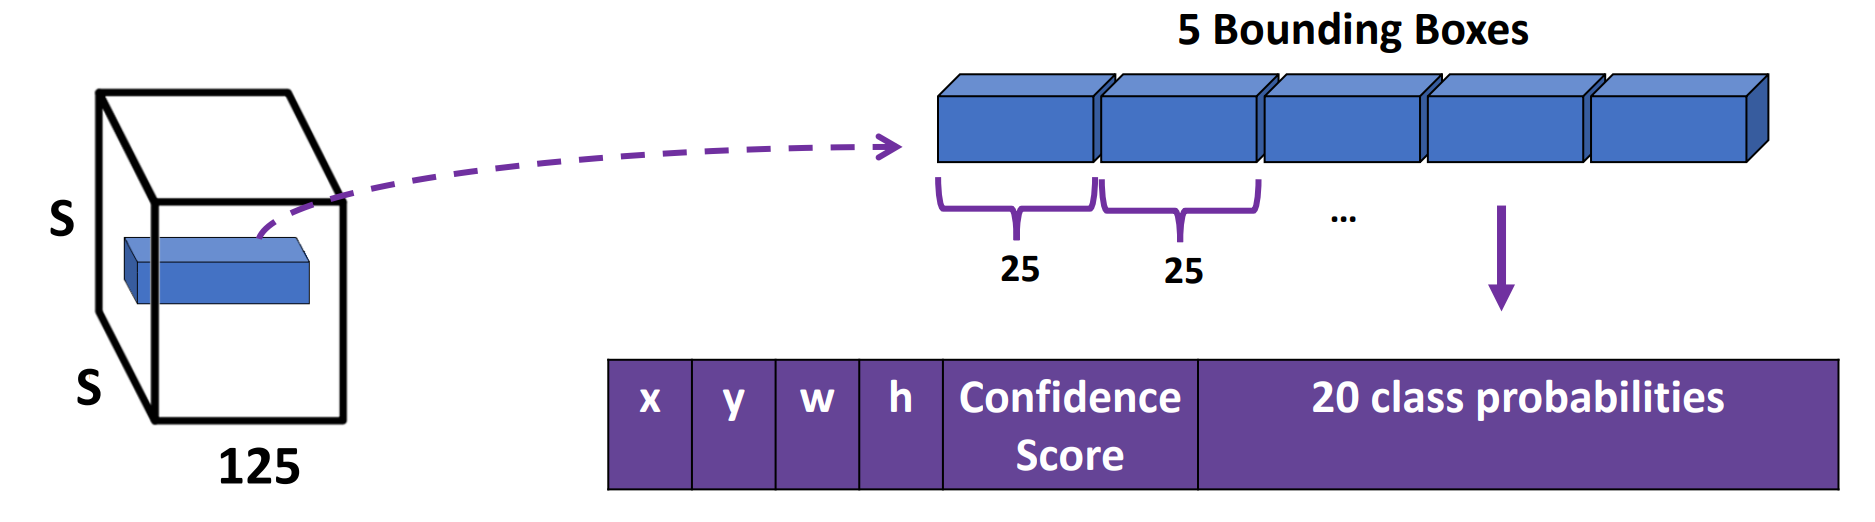
\includegraphics[width=0.78\textwidth,height=0.55\textheight,keepaspectratio]{images/object-detect/yolo_17.png}
        \caption*{\tiny Source: WAIC DL4CV, ``Object Detection and Segmentation'' (Yariv, 2022), sl. 35; image: Redmon \& Farhadi, ``YOLO9000'', CVPR 2017}
    \end{figure}    
\end{frame}